\appendices

\section{Proof of Transit Factor for Manhattan Grid Network}

We outline a simple proof for determining the transit factor of the center node in a Manhattan grid topology of $N$ nodes using "Row-First, Column-Second`` routing, not including traffic originating or ending at the center node.  

Assume that each node is the source of exactly one flow at all times and that the destination of this flow is uniformly chosen from all other $N-1$ nodes in the network.  Node $i$, then, has a $\frac{1}{N-2}$ chance of choosing each other node that is not the center of the grid.  For each source node, we can determine the number of destinations that route through the center.  We separate nodes into two categories for this counting.

\begin{figure}
\begin{centering}
    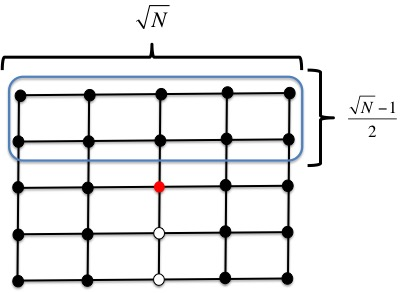
\includegraphics[scale=0.50]{figures/TF_proof_fig_1.jpg}
    \caption{Possible destinations for source nodes in set $A$}
    \label{fig:TF_proof_fig_1}
\end{centering}
\end{figure}

The first set of nodes we consider are those circled in Figure \ref{fig:TF_proof_fig_1}.  We will call these nodes set $A$.  Through manual inspection, one can deduce that the only destination nodes in the figure that result in a path that is relayed by the center node are the white-colored nodes.  We define the probability of a node in set $A$ choosing one of these destinations from all possible destinations as
\begin{equation}
	P_{A} = \frac{\frac{\sqrt{N}-1}{2}}{N-2}
\end{equation}
Now, we can count the total number of nodes for which this probability holds.  From the figure, we can quantify the number of circled nodes, but we must also consider the reverse, i.e. imagine the figure rotated vertically, so the total number of nodes falling into set $A$ is actually
\begin{equation}
	N_{A} = \sqrt{N}*(\sqrt{N}-1)
\end{equation}

Then, the expected number of paths being forwarded by the center node at any given time by nodes in set $A$ is simply the product of $P_A$ and $N_A$:
\begin{equation}
	E[TF_{A}] = \frac{\frac{\sqrt{N}-1}{2}}{N-2} * \sqrt{N}*(\sqrt{N}-1)
\end{equation}

\begin{figure}
\begin{centering}
    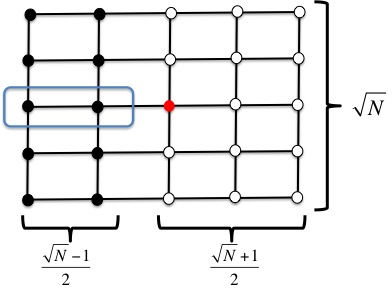
\includegraphics[scale=0.50]{figures/TF_proof_fig_2.jpg}
    \caption{Possible destinations for source nodes in set $B$}
    \label{fig:TF_proof_fig_2}
\end{centering}
\end{figure}

Next, we consider the nodes not in set $A$.  These nodes are in the same row as the center node, and we will call them set $B$, shown as the circled nodes in Figure \ref{fig:TF_proof_fig_2}.  Here, all destinations on the ``opposite" side of the center as well as those in the same column of the center require being routed through the center node when originating from any nodes in set $B$.  Just as above, we can relate the probability of choosing one of these destinations and count the number of nodes in set $B$:
\begin{equation}
	P_{B} = \frac{\frac{\sqrt{N}+1}{2}*m - 1}{N-2}
\end{equation}
\begin{equation}
	N_{B} = 2*(\frac{\sqrt{N}-1}{2})
\end{equation}
The resulting expected transit factor for the center node attributed by nodes in set $B$ is
\begin{equation}
	E[TF_{B}] = \frac{\frac{\sqrt{N}+1}{2}*m - 1}{N-2}*2*(\frac{\sqrt{N}-1}{2})
\end{equation}

Since sets $A$ and $B$ account for all non-center nodes in the network, the overall expected transit factor is just the sum of $E[TF_A]$ and $E[TF_B]$, which simplifies to
\begin{equation}
	E[TF] = \frac{\sqrt{N}(N - 2) + 1}{N-2}
\end{equation}
which is  $O(\sqrt{N})$ for large $N$.



\section{Explanation of Random Variables for Measuring QoI}
First, we explain the expected number of images that are from the same set as the target image in the Top-k algorithm.  We define the following:  

\begin{itemize}
	\item $n$ = total number of images (all sets)
	\item $S$ = number of sets
	\item $S_k$ = set of target image
	\item $k$ = number of images collected
	\item $N_{S}$ = number of images in each set (assumed to be the same here for simplicity)
	\item $x$ = number of images returned $\in S_k$
\end{itemize}

If $k \leq N_{S}$, then 
\begin{equation}
	p(X = x | k) = \frac{{k \choose x} * {n-k \choose k-x} }{ {n \choose k}}, \forall x \leq k
\end{equation}
Otherwise, $p(X = x | k) = 0$.
Comments:  $x$ must be less than $k$ because one cannot choose more items from the target set than are chosen overall.  The probability expression describes the possible combinations of choosing $x$ from the target set and $k-x$ from the $n - N_{S_k}$ remaining images.

If $N_{S} < k < n-N_{S}$, then we consider the possible combination choosing $x$ images from the target set and $k-x$ images from the remaining $n-N_{S}$ images, resulting in the following expression:

$p(X = x | k) = N_{S} choose x * n-N_{S} choose k-x / n choose k$

Finally, when $k > n-N_{S}$, then $k - (n-N_{S} + x)$ images must be from the target set by the pigeonhole principle, so the $p(X = x) = 0$ for all $k > n - N_{S} + x$.  Otherwise, the same expression as directly above is true.


For cluster and spanner, we want to determine the probability that we will cover each of the $S$ sets with at least one of the $k$ chosen images if we had chosen them randomly.  We will call $X_i$ the random variable that represents the number of images from set $i$ in the results.  We use the following expression:

\begin{equation}
	P( X_i > 0 , \forall i) = (1 - P(X_i = 0))^{S}
\end{equation}
where $X_i$ is given by a multivariate hypergeometric distribution, which gives us the following:
\begin{equation}
	P(X_i = 0) = \frac{{n-N_s \choose k}}{{n \choose k}}
\end{equation}